\begin{filecontents*}{example.eps}

gsave
newpath
  20 20 moveto
  20 220 lineto
  220 220 lineto
  220 20 lineto
closepath
2 setlinewidth
gsave
  .4 setgray fill
grestore
stroke
grestore
\end{filecontents*}
%
\RequirePackage{fix-cm}
%
%\documentclass{svjour3}                     % onecolumn (standard format)
%\documentclass[smallcondensed]{svjour3}     % onecolumn (ditto)
\documentclass[smallextended]{svjour3}       % onecolumn (second format)
%\documentclass[twocolumn]{svjour3}          % twocolumn
%
\smartqed  % flush right qed marks, e.g. at end of proof
%
\usepackage{graphicx}
%
% \usepackage{mathptmx}      % use Times fonts if available on your TeX system
%
% insert here the call for the packages your document requires
%\usepackage{latexsym}
% etc.
%
% please place your own definitions here and don't use \def but
% \newcommand{}{}
%
% Insert the name of "your journal" with
 \journalname{Springers}
%
\begin{document}

\title{Maximum Power Point Tracking in Wind Energy Conversion Systems using Machine Learning}
\titlerunning{MPPT IN WECS using Machine Learning}        % if too long for running head
\author{  C. Balakrishna Moorthy\and Siddarth Sreeni\and Sahitya Tahiliani }

\institute{Dr. C. Balakrishna Moorthy\at
              Lecturer, BITS Pilani, K.K. Birla Goa Campus\\
              Tel.: +832 2580229\\
              Mob.:  +919637356896\\
              \email{cbkmoorthy@gmail.com}  \\
           \and
           Siddarth Sreeni \at
	Student, BITS Pilani, K.K.Birla Goa Campus\\
	Mob.: +919400502158\\
             \email{sidda2158@gmail.com}  \\
	\and
	Sahitya Tahiliani \at 
	Student, BITS Pilani, K.K.Birla Goa Campus\\
	Mob.: +917038950104\\
	\email{tsahitya105@gmail.com}}

\date{Received: date / Accepted: date}
% The correct dates will be entered by the editor
\maketitle
\begin{abstract}
    In this paper, an efficient and feasible algorithm to extract the maximum power point (MPP) in wind energy conversion systems (WECS) by implementing machine learning (ML) into perturb and observe (P\&O) algorithm is presented. The proposed algorithm is simulated on a separately-excited DC generator. This model uses instantaneous measurements of wind speed, humidity, temperature, pressure and generator speed to estimate a MPP by using ML at the end of each iteration. From this estimated power point, the controller follows quick perturbation to calculate the accurate MPP and is used as training data for further predictions in the next iteration. The controller learns from this training set and estimates the MPP closer to the maximum achievable power (MAP) which is corrected again through perturbation and is recorded. With the progress of time, the approximation of the maximum power point becomes more accurate whilst the time in further perturbation required for modification decreases. This model adapts to the versatile climatic conditions and yields an efficiency of 99.95\% in predicting the MAP at the end of 1000 iterations corresponding to 2 hours 30 minutes.
\keywords{Wind energy conversion systems \and Maximum power point tracking \and Perturb and Observe \and  Artificial Intelligence \and Machine Learning }
\end{abstract}
\section{Introduction}
\label{intro}
Majority of the energy requirements in today’s world are met with fossil fuels which are costly, non-renewable and pollute the environment. There is a necessity to switch to green energy resources. A lot of research is carried out in this area to find alternative energy resources that are renewable and can be easily harnessed. Such existing resources are solar and wind energy. Wind energy is a good alternative and is environmental friendly. Almost all regions throughout the world receive enough wind to produce energy on a large scale. Wind energy conversion systems (WECS) are of major importance in recent days \cite{RefJ1}. There is a  need to optimise the process of harnessing wind energy. An effective mechanism is thus required to efficiently harness maximum wind energy power. Since wind speed is continuously changing, it is difficult to extract a continuous and maximum power. Hence, there is a need for WECS to be carried out efficiently. An efficient and cost-effective system for capturing the maximum power is required. WECS consists of a wind turbine, charger controllers and an inter-connection apparatus to supply the generated power from the wind to the transformers for further distribution. During windy periods, the wind cuts the blades of the turbine and causes the blades to rotate which in turn generates a torque Wind energy power output can be analyzed based on the Power (P)- current (I) curve. The power-current characteristics under different wind speeds are shown in Figure \ref{Figure:1}.
\begin{center}
\begin{figure}
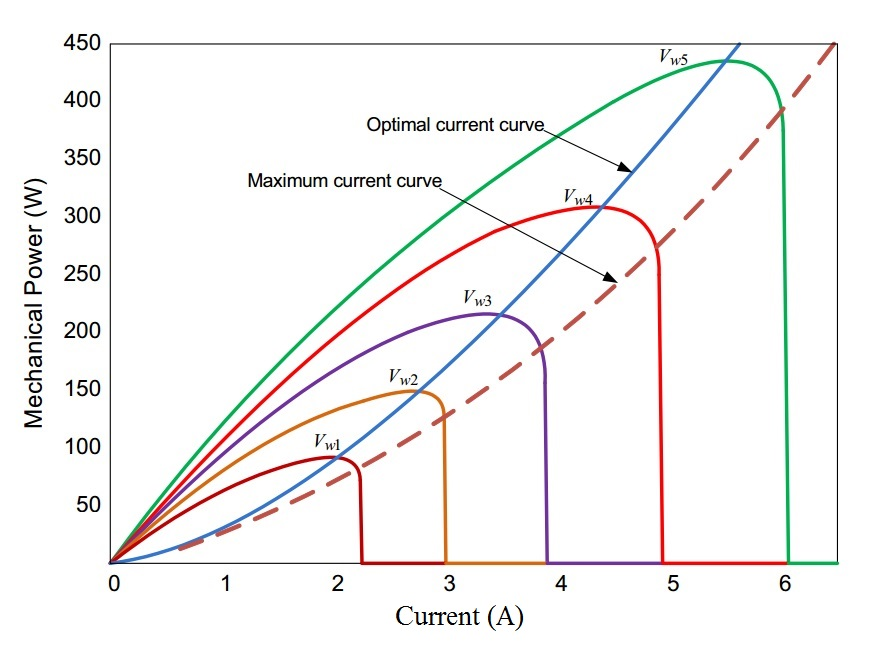
\includegraphics[width=12cm,keepaspectratio]{1.png}
\caption{The Power-Current graph under constant wind speed.\cite{RefJ2}}
\label{Figure:1}    
\end{figure}
\end{center}
A load impedance is required for the generator to change the values of current and thus track the maximum power at different wind speeds. Since the graph plotted keeps shifting from its original position as the wind speed is changing continuously, this fluctuates the peak point of power. Therefore, the load impedance is required to be updated again to get the maximum power characteristic values for voltage and current. The process is known as maximum power point tracking (MPPT). MPPT is carried out by designing efficient charger controllers for extracting maximum power from WECS. The charger controller is designed to control and optimize the generated power. Various methods like perturb and observe (P\&O) \cite{RefJ3}, method of incremental conductance \cite{RefJ4}, method of fractional voltage\cite{RefJ5}, neural network \cite{RefJ6} and fuzzy logic control \cite{RefJ7}, etc., are  used in a charger controller to generate efficient power outputs. These algorithms have been compared on the basis of complexity, efficiency, performance, etc., are listed in Table \ref{Table:1}.
\begin{table}
% table caption is above the table
\label{Table:1}       % Give a unique label
% For LaTeX tables use
\caption{ Comparison of  different MPPT techniques \cite{RefJ6}}
\begin{tabular}{lllll}
\hline\noalign{\smallskip}
Technique & Convergence Speed & Complexity &Tuning & Parameters  \\
\noalign{\smallskip}\hline\noalign{\smallskip}
Peturb and Observe & Varies & Low &  No & Voltage \\
Incremental Conductance  &  Varies & Medium & No & Voltage,Current \\
Fractional Voltage & Medium & Low & Yes & Voltage \\
Fractional Current & Medium & Medium & Yes & Current \\
Fuzzy Logic Control & Fast & High & Yes & Varies \\
Neural Network & Fast & High & Yes & Varies \\
\noalign{\smallskip}\hline
\end{tabular}
\end{table}
In this paper, an alternative approach to overcome the limitations of existing methods is described. The proposed design uses machine learning (ML) into perturb and observe to estimate the maximum power point (MPP). ML is a type of artificial intelligence that provides system the ability to learn without manually programming. It focuses on the developing software programs that can learn on its own and vary on exposure to new set of data. Results have been compared with the existing methods on the basis of efficiency and performance.
\section{System Model}
\label{sec:1}
Figure \ref{Figure:2}. describes the functioning of the proposed wind energy conversion system.The system comprises of a buck converter is coupled with a DC generator. This acts as a DC to DC converter that controls the proportion of input to output voltage by a pulse wiidth modulation (PWM) signal via charger controller.
\begin{center}
\begin{figure}
 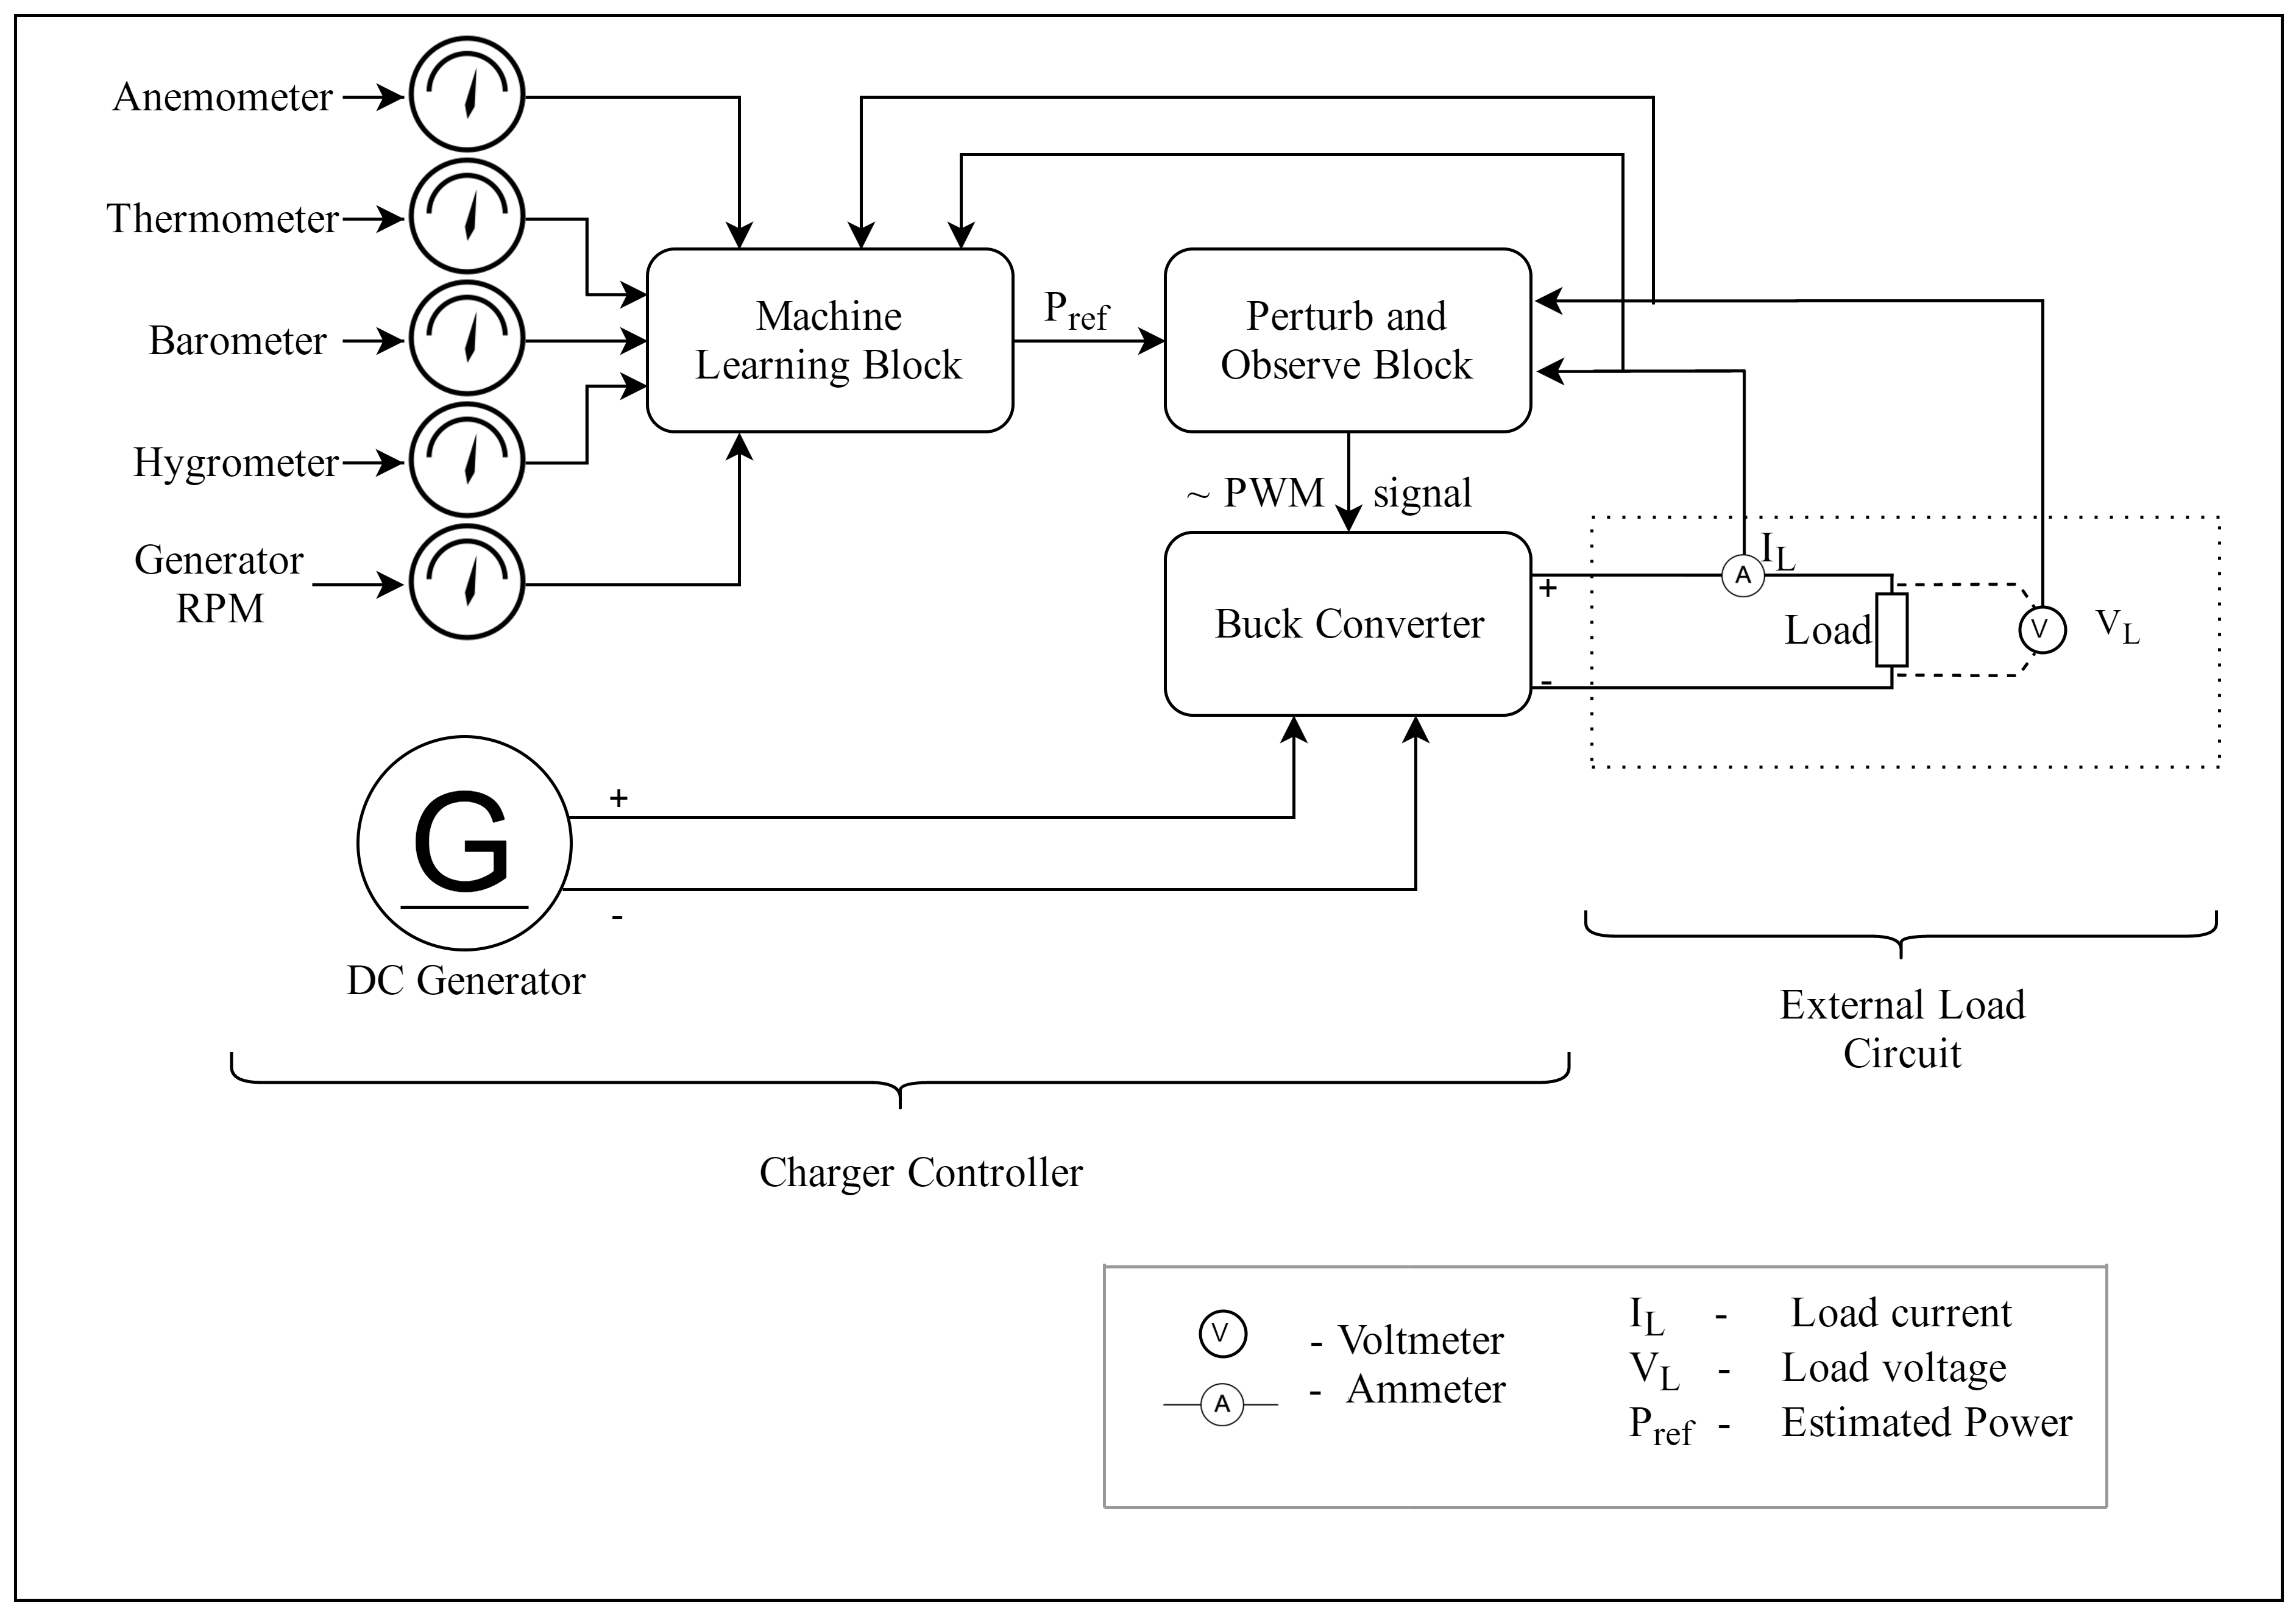
\includegraphics[width=12cm,keepaspectratio]{2.png}
\caption{The configuration of wind energy conversion system.}
\label{Figure:2}    
\end{figure}
\end{center}
\subsection{Separately excited DC generator Model:}
The wind energy conversion system transforms the mechanical energy into electrical energy. The mechanical power $(P_m$) fed to the wind turbine is described as kinetic energy (KE) of the wind turbine rotor blade per unit time (t) \cite{RefJ8} :
\begin{equation} \label{eq:1}
P_m =\frac{KE}{t} = \frac{1}{2} \rho  Av^3
\end{equation}
where, $\rho$ is the air density, $A$ is the area covered under the rotor blade ,$v$ is the wind speed (m/s). ). This is ideal power fed to the wind turbine. But there is a theoretical limit to which this power can be utilized in practice. This limit is governed by Betz’s law\cite{RefJ9} which illustrates the maximum power that can be extracted from the wind turbine, independent of its design. According to the Betz's law, no turbine can capture greater than 59.3\% of the kinetic energy of the wind. The generated power by the wind turbine depends on the efficiency factor, also known as coefficient of  performance  $C_p$($\lambda$, $\beta$) of the wind turbine which depends on pitch angle ($\beta$) and tip speed ratio ($\lambda$). The tip speed ratio is the ratio of  the turbine speed to the wind speed and is given by:
\begin{equation} \label{eq:2}
\lambda=\omega \frac{R}{V}
\end{equation}
where, $\omega$  is the angular speed of the turbine and R is the radius of the turbine. Hence the actual power ($P$) generated by the wind turbine as follows:
\begin{equation} \label{eq:3}
P=C_p(\lambda,\beta)P_m = \frac{1}{2}C_p(\lambda,\beta) \rho  Av^3
\end{equation}
The coefficient of  performance has a maximum value of 0.593. The turbine’s coefficient of performance is a nonlinear function and is expressed by \cite{RefJ10}:
\begin{equation} \label{eq:4}
C_p(\lambda,\beta) = 0.5 ( 116 \frac{1}{\lambda_i} - 0.4 \beta - 5) e^\frac{-21}{\lambda_i}
\end{equation}
Where, $\beta$ is the pitch angle and $1/\lambda_i$ is: 
\begin{equation} \label{eq:5}
\frac{1}{\lambda_i} = \frac {1}{\lambda + 0.08 \beta} - \frac{0.035}{1+\beta^3}
\end{equation}
The characteristic curve for coefficient of  performance $C_p$($\lambda$, $\beta$) versus tip speed ratio ($\lambda$) for various values of the pitch angle ($\beta$) is shown in Figure \ref{Figure:3}.
\begin{center} \begin{figure}
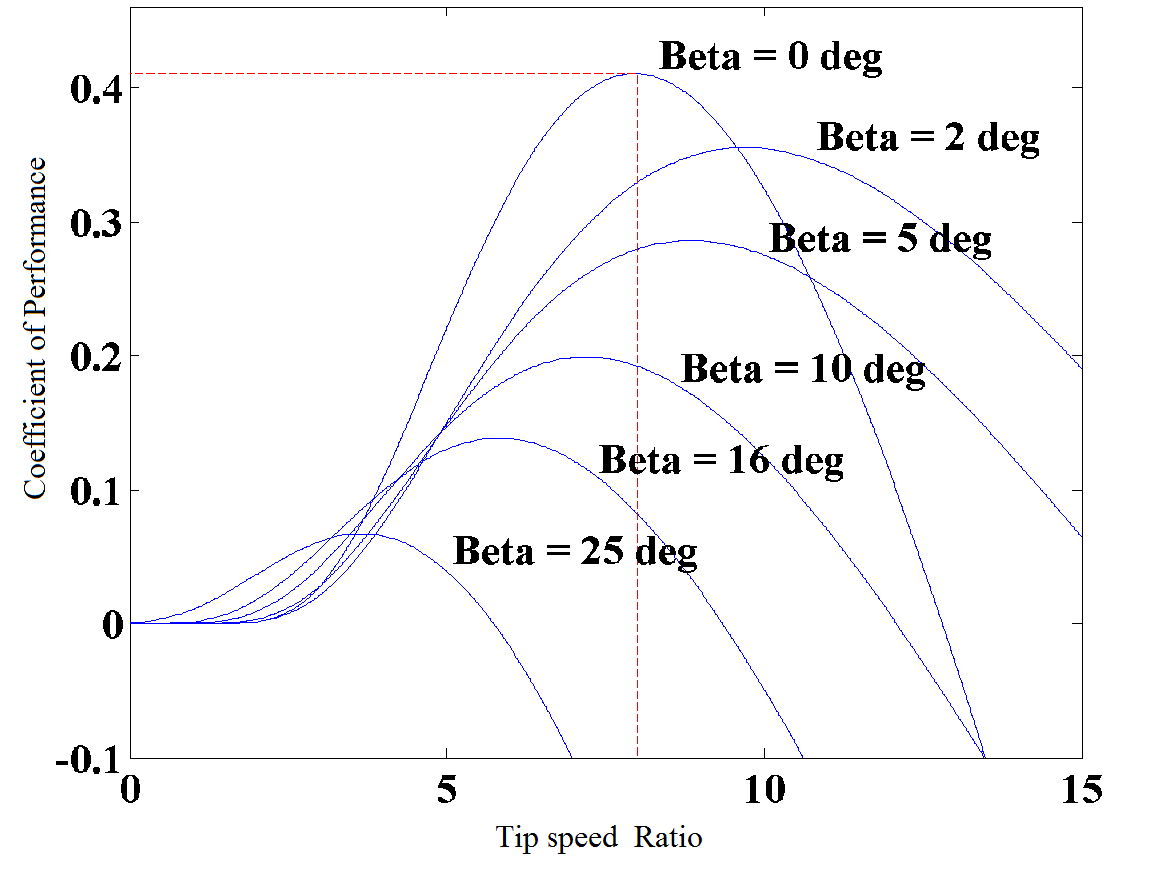
\includegraphics[width=12cm,keepaspectratio]{3.png}
\caption{$C_p(\lambda,\beta)$ vs $\lambda$ characteristic curve for different $\beta$. \cite{RefJ11}}
\label{Figure:3}    
\end{figure} \end{center}
\subsection{Buck Converters}
A Buck Converter\cite{RefJ12} is a DC-to-DC converter that steps down voltage whilst increasing current from its input supply to its output load.This device is essentially a switched-mode power supply typically containing at least two semiconductors (a transistor and a diode), a minimum of one capacitor, inductor or a combination of both and is used for stepping down DC voltage. A PWM signal is used for controlling the clock cycles of the stepping-down operation. A buck converter circuit is shown in Figure \ref{Figure:4}.
\begin{center}
\begin{figure}
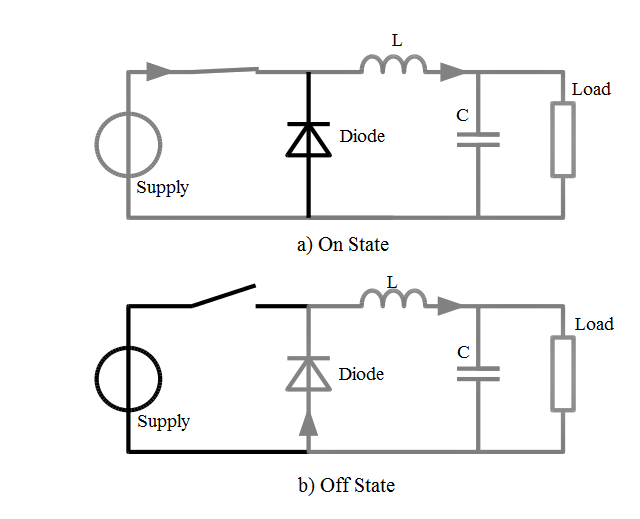
\includegraphics[width=12cm,keepaspectratio]{4.png}
\caption{ A circuit showing modelling of buck converters  \cite{RefJ12}}
\label{Figure:4}    
\end{figure}
\end{center}
\subsection{Peturb and Observe}
Perturb and Observe (P\&O) algorithm is the most simple and efficient method for MPPT in wind-energy conversion systems \cite{RefJ13}, \cite{RefJ14}. In this method, a controller adjusts the output power of the separately excited DC generator by controlling the duty cycle (PWM) of the buck converter, and measures the rise and fall in power continuously. If there is an increment in the power on increasing the duty cycle, then the duty cycle is increased further in the same direction. If there is a decrement in power, then the direction is reversed and the process is repeated in the opposite direction until there is no further rise in power. Hence the characteristic parameters of this point being the maximum power point are recorded and the optimum power is generated using them. This algorithm is frequently used in wind power generation due to its ease of implementation. A flow chart depicting P\&O algorithm using buck convertors has been shown in Figure \ref{Figure:5} where $ P_i$ is the calculated power in the current iteration and $P_{i-1}$ is the power of the preceding iteration.
\begin{center}
\begin{figure}
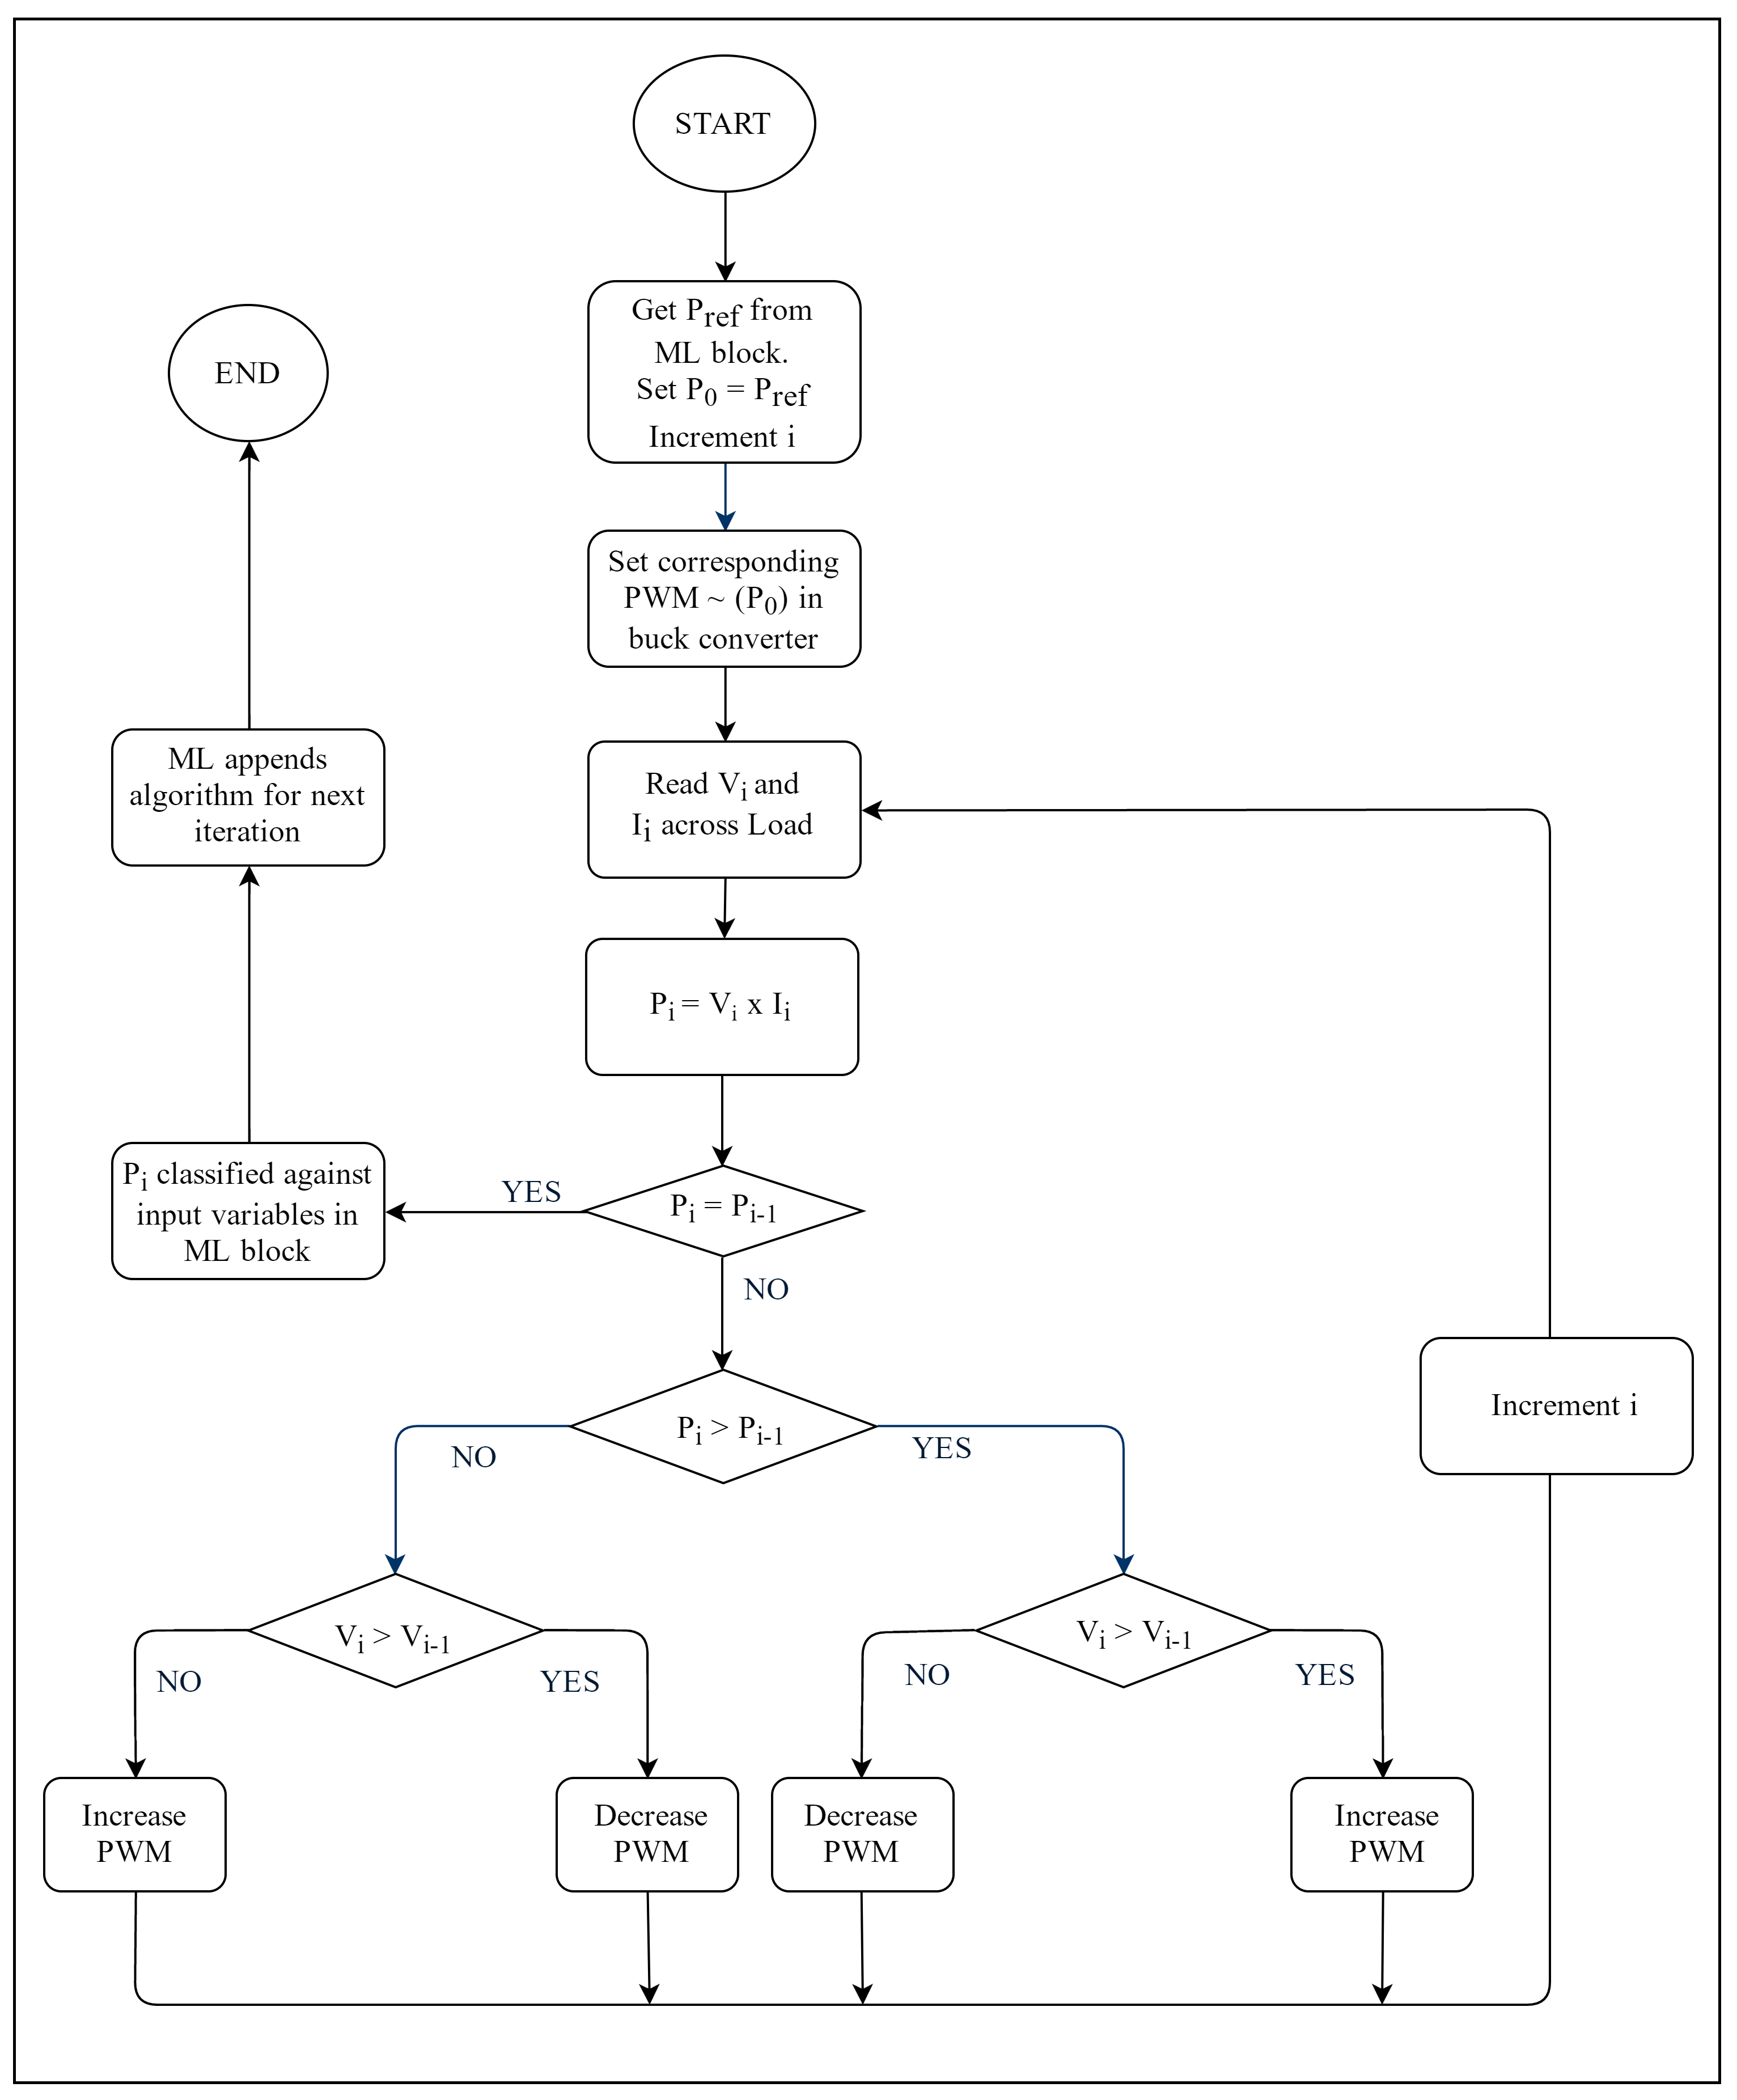
\includegraphics[width=12cm,keepaspectratio]{5.png}
\caption{Flowchart depicting P\&O algorithm}
\label{Figure:5}    
\end{figure}
\end{center}
\subsection{MPPT Algorithm}
The proposed method is a modified approach to Perturb and Observe algorithm. The process of Machine Learning (ML) is similar to data mining, however the obtained results and conclusions from the older data are used to estimate results for the new data. Hence, an artificial intelligent supervised learning technique is used in this paper. The machine learning algorithm used in this model estimates a power point close to the maximum achievable power(MAP). It uses a localised linear regression model based on characteristic parameters ($b_i$ as given in equation \ref{eq:7}) of previously observed MPP(s) and current wind speed, humidity, pressure, temperature, and generator RPM. The proposed system is a causal system. This model generates an algorithm and recognizes patterns in the formation of the MPP(s). As time progresses, the feedback updates the estimation algorithm. The system recognizes more patterns and refines the regression model parameters as in equation \ref{eq:7} and equation \ref{eq:8}. 
\begin{equation} \label{eq:6}
\phi_t =F_t( \phi_0 .... \phi_{t-1}) 
\end{equation}
Here $\phi(t)$ is the MPP at time $t$.The ML algorithm is represented as $F_t$  for ease of understanding. It is the estimation function at time $t$ using the dataset of MPP(s) at previous iterations ($ \phi_0 .... \phi_{t-1}$) and the characteristic variables as in equation \ref{eq:7}. The obtained result is passed on to the next block as $ P_{ref}$ and from here the algorithm follows regular P\&O to obtain the MPP $(P_t)$ using a synchronous Buck DC - DC convertor. A linear regression model is generalized by the following formula. The prediction of $Y_i$ is computed by equation \ref{eq:7} \cite{RefJ15}.
\begin{equation} \label{eq:7}
Y_i= b_0 + b_1 X_{1i} + ... + b_k X_{ki} + \varepsilon_i 
\end{equation}
Where $b_i$ are the regression coefficients, $X_{ik}$ are the regressor variables or the input variables and $\varepsilon_i$ is the error at iteration $i$.  $Y'$ is the mean of all the predicted values of Y (MPP) using variable inputs $ X_{ik}$ and with $ k$ predictor variables. The $b$ values are called regression weights and are computed in order to minimize the sum of squared deviations as shown in equation \ref{eq:8}.
\begin{equation} \label{eq:8}
\sum_{i= 1 }^{N} (Y_i - Y'_i)^2
\end{equation}
Here $N$ is the number of iterations. 
\section{Experimental Results}
A graph between maximum available power (MAP) and predicted MPP is shown in Figure \ref{Figure:6}.
\begin{center}
\begin{figure}
\includegraphics[width=12cm,keepaspectratio]{6.png}
\caption{Comparison of estimated Power $\phi_t$ (blue) and maximum available power (MAP) $P_t$ (red)}
\label{Figure:6}    
\end{figure}
\end{center}
The prediction of function $F_t$  to the MAP $\phi_t$ is much more accurate than $ F_{t-1}$. Figure \ref{Figure:7} shows the mean error in estimating the MPP after each iteration. It is evident that the error is decreasing. After each iteration, the system tries to fits more patterns and the error obtained decreases with time. Hence the system learns.
\begin{center}
\begin{figure}
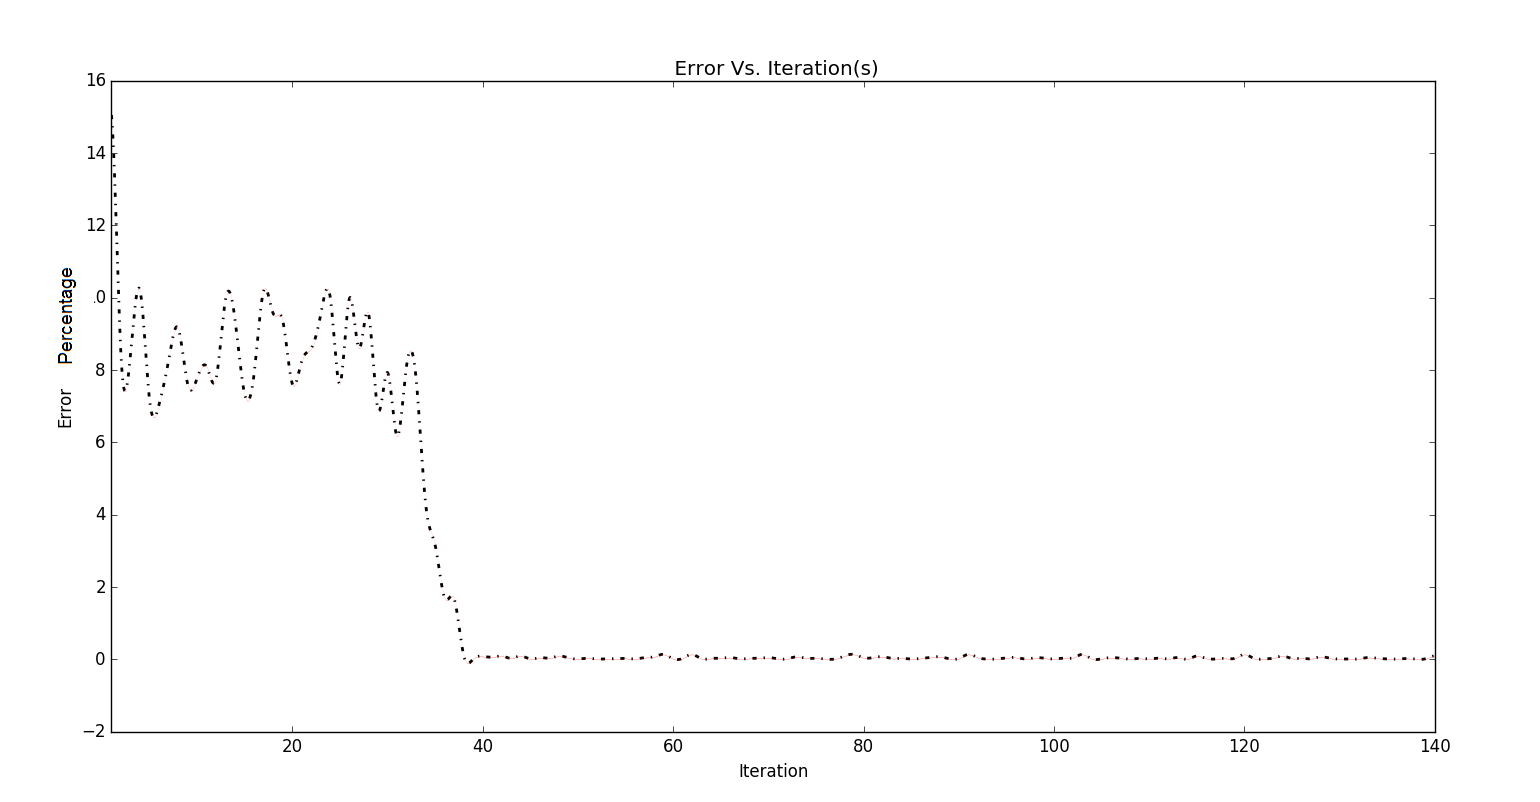
\includegraphics[width=12cm,keepaspectratio]{error.png}
\caption{Mean error at each iteration}
\label{Figure:7}    
\end{figure}
\end{center}
From figure \ref{Figure:8}, the  efficiency of the proposed MPPT model at 1000 iterations which corresponds to $2$ hours $30$ minutes, is greater than 99.95\% for estimating the MPP. Hence, the proposed MPPT algorithm is highly adaptive, efficient and effective. Where the percentage error ($\Delta$) is as follows: 
\begin{equation} \label{eq:9}
\Delta  = 100| ( \frac{P_t - \phi_t}{P_t})|\%
\end{equation}
\begin{center}
\begin{figure}
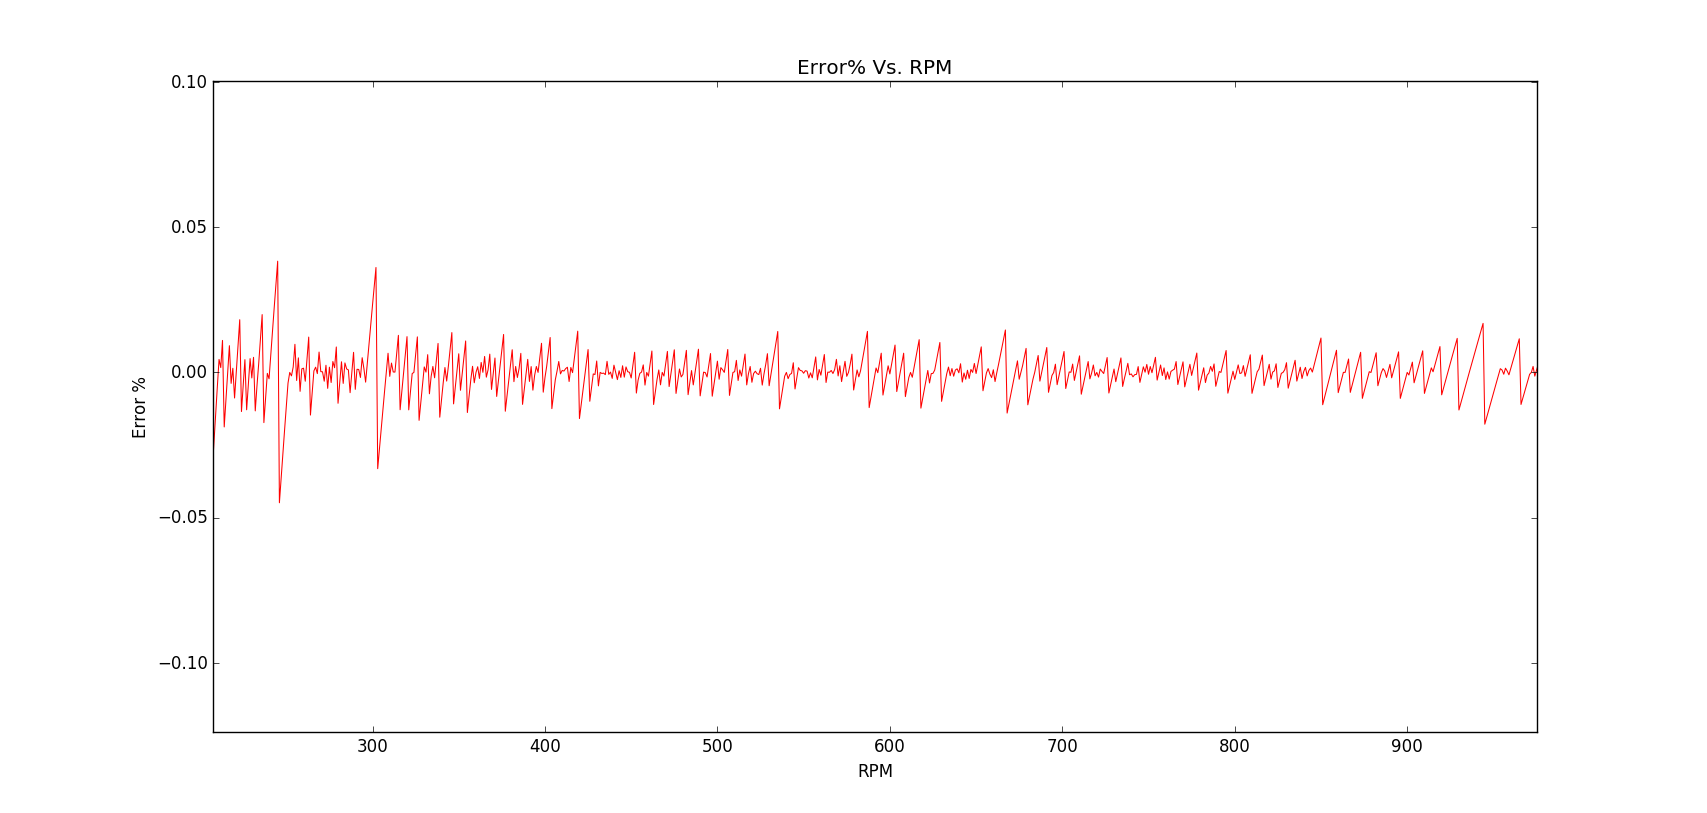
\includegraphics[width=12cm,keepaspectratio]{7.png}
\caption{ Percentage error at each RPM of the DC generator at time $t = 2.5$ hours or $1000$ iterations}
\label{Figure:8}    
\end{figure}
\end{center}
The figures \ref{Figure:9} and \ref{Figure:10} shows the dynamic responses of the generated voltage and current obtained from the proposed MPPT algorithm with respect to time. In this domain,  a validation dataset obtained from P\&O is fed back, after each iteration into the training data, this limits the errors from increasing. Thus, machine learning overcomes overfitting that usually occurs in other AI algorithms such as artificial neural networks (ANN) and other logic based control systems.
\begin{figure}
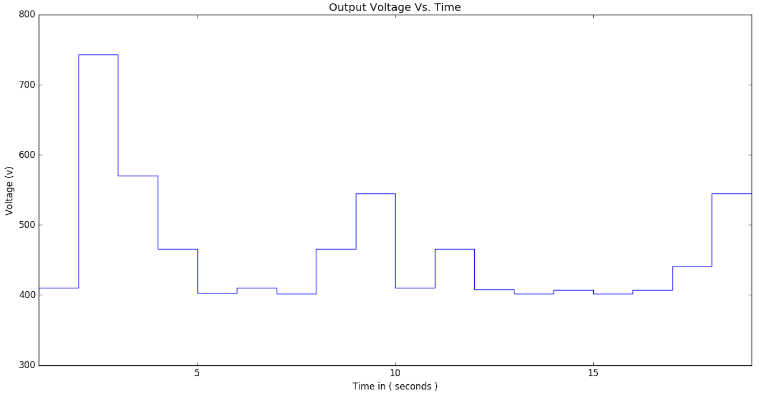
\includegraphics[width=12cm,keepaspectratio]{8.png}
\caption {Output Voltage based MPPT control}
\label{Figure:9}    
\end{figure}
\begin{center}
\begin{figure}
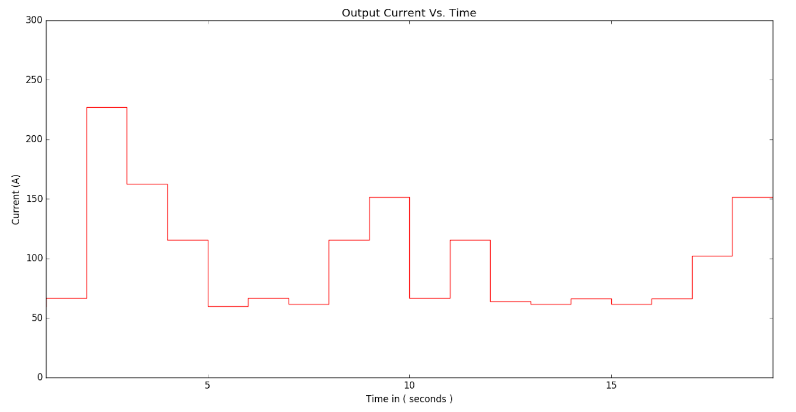
\includegraphics[width=12cm,keepaspectratio]{9.png}
\caption {Output Current based MPPT control}
\label{Figure:10}    
\end{figure}
\end{center}
The above figures show the advantages of using machine learning into perturb and observe. The estimation technique implemented overcomes many of the issues faced in existing MPPT algorithms. These include higher efficiency, faster convergence, ease of implementation and higher precision in estimation
\begin{equation} \label{eq:10}
\eta_t  = (100 - \Delta_{max}^t)\%
\end{equation}
\section{Conclusion}
 In this paper, a highly intelligent method to track maximum power point under varying weather conditions is described. A Python based simulation of a wind energy conversion system with a DC load has been carried out to validate the proposed MPPT method. The results showed that the proposed MPPT method tracked the MPP with negligible oscillations. Observations show that the performance and accuracy of the proposed method is not influenced by the variations in load at all. The perturbation time increases during unexpected wind speeds, but the proposed algorithm gradually learns and adapts to the new weather conditions. The main advantages of the proposed MPPT control method are faster convergence to the MPP, higher efficiency, robustness and its possibility for easy implementation. The system is a modified algorithm of P\&O and can be cascaded to the existing P\&O equipment with convenient setup and thus, resulting in better efficiency.
\begin{thebibliography}{}
\bibitem{RefJ1}
B. K. Sovacool, “The importance of comprehensiveness in renewable electricity and energy-efficiency policy,” Energy Policy, vol. 37, no. 4, pp. 1529-1541, 2009
\bibitem{RefJ2}
K. Chatterjee and D. Kumar, “A review of conventional and advanced MPPT algorithms for wind energy systems,” Renewable and Sustainable Energy Reviews, vol. 55, pp. 957-970, Mar.2016.
\bibitem{RefJ3}
M. A. Elgendy, B. Zahawi, and D. J. Atkinson, “Evaluation of perturb and observe MPPT algorithm implementation techniques,” $6^{th}$ IET International Conference on Power Electronics, Machines and Drives (PEMD 2012), 2012. Control (ICSC), 2016.
\bibitem{RefJ4}
T. Boutabba, S. Drid, L. Chrifi-Alaoui, M. Ouriagli, and M. E. H. Benbouzid, “SPACE real-time implementation of maximum power point tracking based on ripple correlation control (RCC) structure for photovoltaic system,”  $5^{th}$ International Conference on Systems and Control (ICSC), 2016.
\bibitem{RefJ5}
S. M. Ferdous, M. A. Mohammad, N. Farhan, A. M. Saleque, and M. A.Z.M.Shahriar, “Design and simulation of an open voltage algorithm based maximum power point tracker for battery charging PV system,”  $7^{th}$ International Conference on Electrical and Computer Engineering, 2012.
\bibitem{RefJ6}
T. Esram, E. Trishan, and P. L. Chapman, “Comparison of Photovoltaic Array Maximum Power Point Tracking Techniques,” IEEE Trans. Energy Convers., vol. 22, no. 2, pp. 439-449, 2007
\bibitem{RefJ7}
I. H. Altas, Fuzzy Logic Control in Energy Systems with MATLAB. 2017.	
\bibitem{RefJ8}
A. Soetedjo, S. Aryuanto, L. Abraham, and W. P. Mulayanto, “Modeling of wind energy system with MPPT control,”  International Conference on Electrical Engineering and Informatics, 2011.
\bibitem{RefJ9}
A. Betz, Introduction to the Theory of Flow Machines. Elsevier, 2014.
\bibitem{RefJ10}
M. Azzouz, A. Maher, E. Abdel-Latif, and E. Hasan, “Adaptive critic design-based regulation of the DC-bus voltage in wind energy conversion systems,” $49^{th}$ IEEE Conference on Decision and Control (CDC), 2010.
\bibitem{RefJ11}
Zou, Y., Elbuluk, M, \& Sozer, Y. (2010, October)."A complete modeling and simulation of induction generator wind power systems".Industry Applications Society Annual Meeting (IAS), 2010 IEEE (pp. 1-8). IEEE.
\bibitem{RefJ12}
M. Brown and B. Marty, “Switching Power Supply Topologies,” Practical Switching Power Supply Design, 1990, pp.17-42.
\bibitem{RefJ13}
E. Koutroulis and K. Kalaitzakis, “Design of a maximum power tracking system for wind-energy-conversion applications,” IEEE Trans. Ind. Electron., vol. 53, no. 2, pp. 486-494, 2006.
\bibitem{RefJ14}
H. Gitano, G. Horizon, T. Soib, and K. Mohammad, “Design and Testing of a Low Cost Peak-Power Tracking Controller for a Fixed Blade 1.2 kVA Wind Turbine,”  Compatibility in Power Electronics, 2007.
\bibitem{RefJ15}
T. Hill, P. Lewicki, and P. Lewicki, Statistics: Methods and Applications : a Comprehensive Reference for Science, Industry, and Data Mining. StatSoft, Inc., 2006.
\end{thebibliography}
\end{document}


